% -------------------------------------- %
% Bachelor Thesis 2022 - Matteo Alberici
% -------------------------------------- %
\documentclass[]{usiinfbachelorproject}

% Packages
\usepackage[dvipsnames]{xcolor}
\usepackage{algorithm, algpseudocode, enumitem, minted}

% Definitions
\algdef{S}[FOR]{ForEach}[1]{\algorithmicforeach\ #1\ \algorithmicdo}
\algnewcommand\algorithmicforeach{\textbf{for each}}
\captionsetup{labelfont={bf}}

% Document Properties
\author{Matteo Alberici}
\title{SAT-based Techniques for Approximate Circuit \vspace{0.2cm}\\ Design}
\versiondate{\today}

% Committee
\begin{committee}
    \advisor[Universit\`a della Svizzera Italiana, Switzerland]{Prof.}{Laura}{Pozzi}
    \assistant[Universit\`a della Svizzera Italiana, Switzerland]{Dr.}{Ilaria}{Scarabottolo}
\end{committee} 

% ----------------------- %
% Abstract and First Page
% ----------------------- %
\abstract{
As energy efficiency becomes a crucial concern in digital applications, Approximate Computing (AC) has gained popularity, since it represents a potential answer to this ever-growing energy quest. AC brings a new perspective on digital circuit design by adding accuracy to the set of design metrics: it allows slight accuracy reduction in exchange for a significant improvement in energy consumption. AC is particularly suited for error-resilient applications, where such minor accuracy losses do not significantly reduce the quality of the result. In particular, we are interested in Approximate Logic Synthesis (ALS), which is the process of automatically generating, given an exact circuit and a tolerated error threshold, an approximate circuit counterpart where the error is assured to be lower than the specified threshold. The resulting circuit will be a functional modification of the original circuit, where some parts will be substituted or perhaps entirely removed. While several design algorithms have been proposed, we investigate innovative SAT-based solutions. In computer science, multiple problems can be reduced to the SAT problem, including the approximate circuit design challenge investigated here.
}

\begin{document}

\maketitle
\tableofcontents

\newpage

% ----------------------- %
% Chapter 1: Introduction
% ----------------------- %
\section{Introduction}\label{sec:introduction}

% 1.1 - Project Context
\subsection{Project Context}\label{subsec:project-context}
% 1.1.1 - Definition of Approximate Computing
\subsubsection{Definition of Approximate Computing}\label{subsubsec:approximate-computing}
\textit{Approximate Computing} (AC) \cite{als} is an emerging paradigm that improves design area and power consumption by loosening the requirement for total accuracy and, instead, returning potentially inaccurate results rather than guaranteed accurate ones. Since performing exact computations in many scenarios requires an enormous amount of resources, AC \cite{acs} provides a way of obtaining gains in both performance and energy consumption, while still achieving results with acceptable precision. The application efficiency is thus improved by leveraging error resilience. AC performs skillfully for applications such as multimedia processing and voice recognition \cite{eta}, wherein the underlying computation has intrinsic resilience to minor errors. These applications are abundant in different fields such as computer vision, machine learning, and signal processing.

% 1.1.2 - Approximate Circuits
\subsubsection{Approximate Circuits}\label{subsubsec:approximate-circuits}
\textit{Approximate circuits} are approximate computing platforms' fundamental hardware building blocks \cite{ast}. Such circuits outperform traditional ones in speed and design area at the cost of a slight loss in computational accuracy. According to a pre-determined set of quality constraints, an approximate circuit is the realization of a logic function that slightly deviates from the original specification.

% 1.1.3 - Automatic Design of Approximate Circuits
\subsubsection{Automatic Design of Approximate Circuits}\label{subsubsec:automatic-design}
In \textit{approximate circuit} design \cite{eta}, a significant challenge resides in automatically synthesizing approximate circuits (i.e., without manually relying on the expertise of designers). The accuracy of the results in approximate circuits is evaluated based on several error metrics such as worst-case error, bit-flip error, or error-rate, that measure the approximate error by comparing the output of the exact circuit against that of the approximate one. Therefore, it is important to automatically generate approximate circuits that, by design, respect the requirements on the error metrics.

% 1.2 - Project Motivation
\subsection{Project Motivation}\label{subsec:project-motivation}
A preliminary phase of this project concerns circuit visualization, which is a powerful instrument for getting insights on approximate circuits. In order to depict a circuit graphically, we use the \textit{dot} tool. This takes a \textit{GV} file textually describing a circuit written using the graph description language \textit{DOT} in input and produces a new file containing its corresponding graphical representation. The output of \textit{dot} is described in detail after introducing the \textit{GV} format in \hyperref[subsubsec:gv-format]{section 3.1.2}. \\
\textbf{Figure ~\ref{fig:simple-pdf-init}} shows the graphical representation of a simple \textit{GV} file. The circuit described in it holds a NOT gate negating the value in input on the left branch,
and an ASSIGN gate renaming the input on the right. Their values are forwarded to an AND gate, which returns the Boolean value \textcolor{ForestGreen}{true} only if both the values in input are \textcolor{ForestGreen}{true}. The circuit will always return \textcolor{red}{false} since the AND gate receives the initial value and its negated value.
\begin{figure}[H]
    \centering
    \includegraphics[width=5cm]{assets/test_02.pdf}
    \caption{Simple file graphical representation obtained with \textit{dot}}
    \label{fig:simple-pdf-init}
\end{figure}

% 1.3 - Project Goals
\subsection{Project Goals}\label{subsec:project-goals}
% 1.3.1 - Implementing Blif2GV Translator
\subsubsection{Implementing a Translator from Blif to GV}\label{subsubsec:translator}
A commonly used text format for circuit description is the \textit{Berkeley Logic Interchange Format} (BLIF). This project's first objective consists of designing and implementing a translator that, given a \textit{blif} file describing a circuit, takes that file in input, processes and parses it, and returns the corresponding \textit{GV} file as output. Both the formats are exhaustively explained in sections \hyperref[subsubsec:blif-format]{3.1.1} and \hyperref[subsubsec:gv-format]{3.1.2}, respectively. Furthermore, the translator should be able to perform other operations after converting the given file, such as removing useless and redundant gates in order to obtain a simpler version of the processed circuit with the same semantical meaning.
% 1.3.2 - Experiments and Analysis with MUS
\subsubsection{Experiments and Analysis with MUS}\label{subsubsec:experiments-and-analysis}
The second part of this project deals with \textit{Minimal Unsatisfiable Subsets} (MUSes), meaning approximate circuits obtained by removing gates from a given circuit through SAT \cite{sat}. We perform experiments with the MUS toolchain, which, given a benchmark in \textit{GV} format, executes a series of operations to create different versions of the given file. Finally, it finds all the possible \textit{MUSes} within a pre-defined timeout value and with respect to a pre-defined error threshold. MUS theory will be illustrated in \hyperref[subsubsec:mus]{section 3.2.3}.

% 1.4 - Results Obtained
% \subsection{Results Obtained}\label{subsec:results-obtained}
% TODO: Synthesis of the results (leave it for later)

\newpage

% --------------------------- %
% Chapter 2: State of the Art
% --------------------------- %
\section{State of the Art}\label{sec:state-of-the-art}
Nowadays, the state of the art provides a variety of works in SAT-based approximate logic synthesis. One of the most recent methods is called the "\textit{MUS-based Circuit Approximation Technique}".
(MUSCAT) \cite{muscat} and generates "valid-by-construction" approximate circuits by inserting cut-points to replace connections between gates by constant values, allowing for subsequent logic minimization. MUSCAT aims to utilize formal verification engines to identify \textit{Minimal Unsatisfiable Subsets} (MUS), determining the maximum number of non-violating cut-points. MUSCAT's solution is optimal with respect to the number of activated cut-points, also providing a guarantee on the quality constraints. The theory behind MUS will be introduced in \hyperref[subsubsec:mus]{section 3.2.3}. \\
Another method among AC's most important and diffuse ones is \textit{And-Inverter Graphs} (AIGs) \cite{aigs}. It is based on rewriting operations that improve performance and ensures the bounds of approximation errors introduced through formal guarantees on error metrics. This synthesis approach is evaluated on various designs to show its usefulness and applicability. The results obtained with AIGs synthesis show comparable quality to manually hand-crafted approximate designs. Furthermore, AIGs are capable of trading off the relative significance of each error metric for a particular application to improve the quality of the synthesized circuits. \\
The last state-of-the-art model we introduce in this section is the \textit{BMF-based Logic Approximate Synthesis} (BLASYS) \cite{blasys}, which presents a novel paradigm to synthesize approximate circuits using modified algorithms for Boolean matrix factorization (BMF). This methodology approximates the truth table of a sub-circuit through BMF to a controllable approximation degree; the factorization results are then used to synthesize a less complex sub-circuit. BLASYS obtains a smooth trade-off between accuracy and circuit complexity, measured by area and energy consumption.

\newpage

% -------------------------------------------- %
% Chapter 3: Project Design and Implementation
% -------------------------------------------- %
\section{Project Design and Implementation}\label{sec:project-design-and-implementation}

% 3.1 - Blif2GV Translator
\subsection{Blif2GV Translator}\label{subsec:blif2gv-translator}
The first part of this report describes the implementation of the \textit{Blif2GV Translator}: an application that offers a clear graphical view of a circuit. This converter inputs a \textit{blif} file holding the textual representation of a Boolean circuit and outputs the corresponding file in GV format. Both the file formats are exhaustively described in sections \hyperref[subsubsec:blif-format]{3.2.2} and \hyperref[subsubsec:gv-format]{3.2.3}, respectively. \\
The entire translator was developed using the \textcolor{blue}{Python} \cite{py} programming language. \\
The following sections offer a detailed explanation of what happens during each execution phase. \\
Since the Blif2GV Translator deals with Boolean circuits, we must introduce a few notions. \textit{Boolean logic} is the branch of algebra in which the values of the variables are the truth values \textcolor{ForestGreen}{true} and \textcolor{red}{false}, usually denoted by the numbers \textcolor{ForestGreen}{1} and \textcolor{red}{0}, respectively. George Boole introduced it in the book "\textit{The Mathematical Analysis of Logic}" [1847]. A Boolean operator is a function that takes binary variables in input, processes them, and returns a single binary output (i.e., either \textcolor{ForestGreen}{1} or \textcolor{red}{0}). Let us analyze the following example, representing an AND operator:
\begin{center}
    \texttt{\textcolor{ForestGreen}{1} $\land$ \textcolor{red}{0} $=$ \textcolor{red}{0}}
\end{center}
Such operations are defined by \textit{truth tables}, wherein the combinations of inputs and the corresponding output are shown.  Given the fact that we could encounter any type of \textit{unary} (i.e., one input - one output) and \textit{binary} (i.e., two inputs - one output) operators while parsing a \textit{blif} file, we should define each possible input(s)-output relation in order to be able to understand each component of a Boolean circuit. Every Boolean operator is exhaustively defined in \hyperref[section:operators]{Appendix A}, along with the corresponding truth table.
% 3.1.1 - Introducing the blif Format
\subsubsection{Introducing the blif Format}\label{subsubsec:blif-format}
The \textit{Berkeley Logic Interchange Format} (BLIF) \cite{blif} represents a logic-level hierarchical circuit in textual form. The term \textit{circuit} refers to a combinational and sequential network of Boolean functions which can be viewed as a directed graph, where each node can be broken up into the following components:
\begin{itemize}
    \item \textbf{Input(s)}
        \vspace{0.2cm} \\
        The set of inputs received by the node; it could consist of a single input, in the case of a unary operator, an ordered pair of inputs, in the case of a binary operator, or a sequence of inputs with no pre-defined limits, in the case of a special operator. In the latter is the case, then the node must be declared in a \hyperref[it:gates]{\texttt{.subckt}}.
    \item \textbf{Operator}
        \vspace{0.2cm} \\
        The operator that processes the input received by the node and returns the corresponding output; it could be a unary operator, such as NOT, a binary operator, such as AND, or a special operator, such as MUX.
    \item \textbf{Output}
        \vspace{0.2cm} \\
        The single output returned by the operator after the latter finishes processing the received input.
\end{itemize}
The file's body is composed of "commands", which are lines that declare logic gates. The circuit nodes are defined by specifying the input(s), the operator, and the output. There exist two different ways of writing such definitions:
\begin{itemize}
    \item \texttt{.subckt}\label{it:gates}
        \vspace{0.2cm} \\
        This kind of definition has the following syntax:
        \begin{center}
            \texttt{.subckt \$<operator> A=<input> [B=<input2> ...] Y=<output>}
        \end{center}
        Every pair \texttt{letter=<name>} but the last one represents an input of the defined node. The following example shows a logical AND gate definition:
        \begin{center}
            \texttt{.subckt \$and g0 g1 g2}
        \end{center}
    \item \texttt{.names}
        \vspace{0.2cm} \\
        This kind of definition has the following syntax:
        \begin{align*}
            &\texttt{.names <input> [<input2> ...] <output>} \\
            &\texttt{<truth-table>}
        \end{align*}
        The operator is defined by the truth table declared in the lines immediately below. A truth table is defined by one or more lines of numbers, each indicating a boolean relation that returns the logic value \textcolor{ForestGreen}{true}. There must be a sequence of non-separated numbers, one for each input, and a number for the output, white-space-separated by the first sequence. The following example shows a logical AND gate definition:
        \begin{align*}
            &\texttt{.names g0 g1 g2} \\
            &\texttt{11 1}
        \end{align*}
\end{itemize}
The following code snippet represents a simple \textit{blif} file.
\begin{minted}[
frame=lines,
framesep=2mm,
baselinestretch=1.2,
bgcolor=white,
fontsize=\footnotesize,
linenos
]{vim}
.model circuit
.inputs g0
.outputs g8
.names $false
.names $true
1
.names $undef
.subckt $assign A=g0 Y=g1
.subckt $assign A=g0 Y=g2
.subckt $not A=g1 Y=g3
.subckt $not A=g3 Y=g4
.subckt $not A=g2 Y=g5
.subckt $and A=g4 B=g5 Y=g6
.subckt $assign A=g6 Y=g7
.subckt $assign A=g7 Y=g8
.end
\end{minted}

% 3.1.2 - Introducing the GV Format
\subsubsection{Introducing the GV Format}\label{subsubsec:gv-format}
A \textit{Graphviz Dot} (\textit{GV}) file \cite{gv} provides the characteristics of a graph and is written using the \href{https://graphviz.org/doc/info/lang.html}{DOT language}. The body of a \textit{GV} file can be broken up into two parts: the nodes declaration and the edges assignment. Each node-declaring line defines a single gate using the following syntax:
\begin{center}
    \texttt{<node\_name> [label="<node\_label>" <style>]}
\end{center}
The name displayed after converting a \textit{GV} file into a pdf is the value of the property \texttt{label}.
Each edge-declaring line defines a link from a source node to a destination node with the following syntax:
\begin{center}
    \texttt{<source\_node> -> <destination\_node>}
\end{center}
The following code snippet represents the \textit{GV} file corresponding to the \textit{blif} file defined at the end of section \hyperref[subsubsec:blif-format]{3.1.1}.
\begin{minted}[
frame=lines,
framesep=2mm,
baselinestretch=1.2,
bgcolor=white,
fontsize=\footnotesize,
linenos
]{vim}
digraph circuit {
    node[style=filled, fillcolor=white, shape=rect, fontname=geneva]
    g0 [label="in0\ng0", shape=circle, fillcolor=white]
    g1 [label="assign\n\ng1", fillcolor=white]
    g2 [label="assign\n\ng2", fillcolor=white]
    g3 [label="not\n\ng3", fillcolor=white]
    g4 [label="not\n\ng4", fillcolor=white]
    g5 [label="not\n\ng5", fillcolor=white]
    g6 [label="and\n\ng6", fillcolor=white]
    g7 [label="assign\n\ng7", fillcolor=white]
    g8 [label="assign\n\ng8", fillcolor=white]
    g8 [label="out0\ng8", shape=doublecircle, fillcolor=white]
    edge [fontname=Geneva, fontcolor=forestgreen]
    g0 -> g1
    g0 -> g2
    g1 -> g3
    g3 -> g4
    g2 -> g5
    g4 -> g6
    g5 -> g6
    g6 -> g7
    g7 -> g8
}
\end{minted}
\textbf{Figure ~\ref{fig:simple-pdf}} shows the graphical representation of this file. The described circuit is more complex than the one seen in section $2$, but has the same semantical meaning: gate $6$ is an AND gate that takes in input the result of two consecutive NOT gates from the left branch and the value of a single NOT gate from the right one; thus, the AND gate will always evaluate to \textcolor{red}{false}.
\begin{figure}[H]
    \centering
    \includegraphics[width=5cm]{assets/test_01.pdf}
    \caption{File graphical representation obtained with \textit{dot}}
    \label{fig:simple-pdf}
\end{figure}
% 3.1.3 - Blif2GV  Algorithm Description
\subsubsection{Blif2GV Algorithm Description}\label{subsubsec:high-level-description}
Since we deal with logic circuits, we need to implement a way of representing a circuit. A circuit object has a set of inputs, a set of outputs, and a set of sub-circuits, and it is created by parsing a \textit{blif} file's header. Moreover, we must design a way of defining the objects a circuit is made of: the sub-circuits. A sub-circuit object has a set of inputs, an operator, and a single output and represents a circuit gate. \\
\textbf{Algorithm ~\ref{algo:blif-parser}} shows the pseudo-code of the parsing method performed by the \textit{Blif2GV Translator}.
\begin{algorithm}[H]
    \caption{\texttt{blif\_parser(file\_name)}}
    \begin{algorithmic}[1]
        \State generate ckt object from file\_name
        \State set subckts to []
        \State open file\_name
        \ForEach{line in file\_name.lines}
            \State create subckt
            \State append subckt to subckts
        \EndFor
        \State close file\_name
        \State assign subckts to ckt
        \State assign children and parents to each subckt
        \State simplify ckt
        \State \textbf{return ckt}
    \end{algorithmic}
    \label{algo:blif-parser}
\end{algorithm}
\noindent
In order to parse \texttt{.name} lines, we must perform a few more operations. \\
In the case of such a line, we need to parse the first line to get the input(s) and the output; then, we must parse the truth table defined in the following lines to assign the corresponding operator. The encounterable truth tables are defined in dictionaries created by permuting each operator definition. As a result, a truth table is identified independently of how it is declared.
% 3.1.4 - Simplifying a Circuit
\subsubsection{Simplifying a Circuit}\label{subsubsec:simplifying-circuit}
After implementing the translator, we wish to program more features to generate more simple circuits. 
\subsubsection*{Fixing the Syntax}
Given that the syntax of a \textit{GV} file rejects several symbols that, in contrast, could be used in a \textit{blif} file, we must modify everything that could lead to an error. More specifically, the \textit{GV} syntax does not accept non-alphanumeric characters at the beginning of a gate name and many special symbols inside it. \\
Let us examine the following example, taken from \textit{BLASYS}:
\begin{center}
    \texttt{.subckt \$and A=\$not\$abs\_.v:164\$307\_Y B=\$not\$abs\_.v:164\$308\_Y Y=\$and\$abs\_.v:164\$309\_Y} \\
    $\Downarrow$ \\
    1) \ input: \texttt{n164\_307\_Y} \ \ operator: \texttt{and} \ \ output: \texttt{n164\_309\_Y} \\
    2) \ input: \texttt{n164\_308\_Y} \ \ operator: \texttt{and} \ \ output: \texttt{n164\_309\_Y} \\
\end{center}
\subsubsection*{Removing Useless ASSIGN Gates}
The role of an ASSIGN gate is renaming the received input and forwarding it to another gate. Since these gates are introduced by \textit{blif} files and do not alter the semantical meaning of the circuit, we decided to remove such gates. We must ensure that each link is set correctly after the removal in order not to get errors. \textbf{Figure ~\ref{fig:simple-pdf-1}} shows the graphical representation of the circuit defined in \textbf{Figure ~\ref{fig:simple-pdf}} after performing the first removal operation: all the ASSIGN gates are removed.
\begin{figure}[H]
    \centering
    \includegraphics[width=3.9cm]{assets/test_01_assign.pdf}
    \caption{ASSIGN gates removal result}
    \label{fig:simple-pdf-1}
\end{figure}
\subsubsection*{Removing Redundant NOT Gates}
A NOT gate changes the value of the input received into its complement (i.e., from \textcolor{ForestGreen}{true} to \textcolor{red}{false} and vice-versa). Two or more NOT gates are redundant if the value outputted by the last gate of the sequence is equal to the value taken in input by the first gate. \\
\textbf{Figure ~\ref{fig:simple-pdf-2}} shows the graphical representation of the circuit defined in \textbf{Figure ~\ref{fig:simple-pdf}} after performing the second removal operation: the redundant NOT gates are entirely removed.
\begin{figure}[H]
    \centering
    \includegraphics[width=3.9cm]{assets/test_01_not.pdf}
    \caption{NOT gates removal result}
    \label{fig:simple-pdf-2}
\end{figure}
% 3.2.7 - Executing the Translator
\subsubsection{Executing the Translator}\label{subsubsec:executing-translator}
There are two different manners for executing the translator: a \textit{Text-based User Interface} (TUI) or a \textit{Graphical User Interface} (GUI).
\subsubsection*{Text-based User Interface}
In order to run the translator with the TUI, it is sufficient to type the following command while being in the project's root directory:
\begin{center}
    \texttt{python3 main.py <blif\_file\_name> [dot]}
\end{center}
The placeholder \texttt{<blif\_file\_name>} must be replaced by the path of the \textit{blif} file that the user wants to convert. Moreover, it is possible to add the argument \texttt{dot} to convert the newly generated \textit{GV} file into a pdf using DOT at the end of the translation process. \\
Depending on the result of the translation process, a different message will be displayed in the standard output. The code handles several types of errors. 
\subsubsection*{Graphical User Interface}
In order to run the translator with the GUI, it is sufficient to execute the python script \texttt{main.py} with no additional arguments while being in the project's root directory:
\begin{center}
    \texttt{python3 main.py}
\end{center}
The script will then display a GUI with the following initial window: \textbf{Figure ~\ref{fig:gui-1}} shows the initial window of the GUI.
\begin{figure}[H]
    \centering
    \includegraphics[width=10cm]{assets/Figure 7 - GUI 1.png}
    \caption{GUI - initial window}
    \label{fig:gui-1}
\end{figure}
\noindent
In the top-center part of the window, there are a text area and a button labeled \textit{Browse}: the user can either type the path to a folder containing at least one \textit{blif} file or search for it by clicking on the button.
If the folder selected by the user contains at least one \textit{blif} file, then the window will display a list of all the \textit{blif} files found in that directory on the left. The window will display an error if the selected folder holds no \textit{blif} files. \\
By clicking on one of the displayed \textit{blif} files, the corresponding line of the list will be highlighted. The window will then display the name of the \textit{blif} file on the left, along with a button labeled \textit{Convert}: if the user clicks on the latter, then the selected \textit{blif} file will be converted to \textit{GV} and pdf. \\
\textbf{Figure ~\ref{fig:gui-7}} shows the window that appears when the input \textit{blif} file is successfully converted to \textit{GV}, and if the corresponding pdf file is succesfully generated by DOT.
\begin{figure}[H]
    \centering
    \includegraphics[width=10cm]{assets/Figure 13 - GUI 7.png}
    \caption{GUI - successful conversions window}
    \label{fig:gui-7}
\end{figure}
\noindent
Finally, depending on the result of the translation process, a different message will be displayed on the window. The code handles several types of errors.

% 3.2 - SAT for Approximate Synthesis
\subsection{SAT for Approximate Synthesis}\label{subsec:sat-smt}
% 3.2.1 - Introduction to SAT Theory
\subsubsection{Introduction to SAT Theory}\label{subsubsec:sat-theory}
The \textit{Boolean satisfiability problem} (SAT) considers a formula containing binary variables connected by logical relations such as OR and AND. It aims to establish whether there is any way to set these variables so that the formula evaluates to \textcolor{ForestGreen}{true}. \\
The \textit{Boolean satisfiability} problem asks whether there exists at least one combination of input variables $x_i \in \{$\textcolor{ForestGreen}{true}, \textcolor{red}{false}$\}$ for which a Boolean formula returns \textcolor{ForestGreen}{true}, i.e. it is \textit{satisfiable}. \\
A \textit{SAT solver} \cite{sat} is an algorithm for establishing satisfiability: it takes a Boolean formula in input and returns \textcolor{ForestGreen}{SAT} if it finds a combination of variables that satisfies it; otherwise, it returns \textcolor{red}{UNSAT}. It may return without an answer if it cannot determine whether the problem is \textcolor{ForestGreen}{SAT} or \textcolor{red}{UNSAT}.
SAT solvers can be classified into two types: \textit{complete algorithms}, which guarantee to return either \textcolor{ForestGreen}{SAT} or \textcolor{red}{UNSAT}, and \textit{incomplete algorithms}, which could return \textcolor{gray}{UNKNOWN}. \\
The first step for solving a SAT problem is converting the formula in input to a standard form known as \textit{conjunctive normal form}, which consists of a conjunction of disjunctions and is more amenable to algorithmic manipulation:
\begin{center}
    $\Phi = (x_1 \lor x_2 \lor x_3)\ \land\ (\neg x_1 \lor x_2 \lor x_3)\ \land\ (x_1 \lor \neg x_2 \lor x_3) \ \land\ (x_1 \lor x_2 \lor \neg x_3)  $
\end{center}
Each term is called a \textit{clause} and combines variables and their complements with OR operators. Clauses are combined via AND operators. In a \textit{conjunctive normal form}, a variable is known as a \textit{literal}. We can characterize a problem based on the number and size of the clauses in the conjunctive normal form: given that a \textit{$k$-clause} contains $k$ variables, then a problem is \textit{$k$-SAT} if all the clauses contain $k$ variables. \\
A solver which finds a solution returns a \textit{certificate} along with it. A certificate is used to check the result with a simpler algorithm: if the solver returned \textcolor{ForestGreen}{SAT}, then the certificate will be a set of variables satisfying the formula; otherwise, the certificate will be a complex data structure depending on the solver. \\
In the \textit{UNSAT problem}, we aim to show that no combination of literals satisfies a given formula: \textit{UNSAT solvers} return as soon as they establish that the formula is UNSAT, but it may take exponential time. In general, SAT-problems are NP-hard.

% 3.2.2 - SAT for Approximate Synthesis
% \subsubsection{SAT for Approximate Synthesis}\label{subsubsec:sat-approximate-synthesis}
% TODO: write some information concerning SAT theory for approximate synthesis

% 3.2.3 - Minimal Unsatisfiable Subsets
\subsubsection{Minimal Unsatisfiable Subsets}\label{subsubsec:mus}
Given an unsatisfiable Boolean formula $\phi$, an unsatisfiable subset of clauses $U$ of $\phi$ is called \textit{Minimal Unsatisfiable Subset} (\textit{MUS}) if every proper subset of $U$ is satisfiable. Moreover, a minimum unsatisfiable subset contains the smallest number of the original clauses required to be still unsatisfiable. The \textit{MUSes} of a Boolean formula serve as explanations for the unsatisfiability of the formula itself. The availability of efficient SAT solvers has aided the development of techniques for finding and enumerating \textit{MUSes}. \\
A generic combinatorial circuit can always be expressed as a Boolean formula. This formula can be manipulated by a SAT solver to obtain an approximate one that slightly deviates from the original. Indeed, with the proper problem formulation, \textit{MUSes} returned by the solver can be interpreted as approximate circuits. \\
The second part of this project deals with finding and enumerating the \textit{MUSes} of a given benchmark through a toolchain that uses a modified version of \textit{MUST} \cite{mus}, then analyzing the area of the smallest MUS found with respect to an error threshold, since designers are interested in the smallest circuit with equal functionality.

\newpage

% -------------------------------- %
% Chapter 4: MUST Results Analysis
% -------------------------------- %
\section{MUST Results Analysis}\label{sec:results}

% 4.1 - Experimental Settings
\subsection{Experimental Settings}\label{subsec:experimental-settings}
Given a set of benchmarks, we must find the maximum number of \textit{MUSes} for each among them, along with their areas. More precisely, we aim at obtaining the MUS representing the smallest approximate circuit with respect to an error threshold (ET) and a timeout value. We decided to set the timeout value to $30$ to limit the execution time. After running the toolchain on a benchmark, we use \textit{yosys} \cite{yosys} to get the minimal area among the newly-created \textit{MUSes}. Since the used \textit{yosys} script requires a \textit{verilog} file \cite{verilog}, we must use the \textit{abc} tool \cite{abc} to convert the blif version of the considered benchmark to the \textit{verilog} format; the command employed is the following:
\begin{center}
    \texttt{abc -c "read\_blif <benchmark>.blif ; write\_verilog <benchmark>.v"}
\end{center}
Finally, given the number of \textit{MUSes} found, the script \texttt{measure\_area\_yosys.py} returns each \textit{MUS}' area value along with the minimal one. The command to use is the following:
\begin{center}
    \texttt{python3 measure\_area\_yosys.py <benchmark>.v <\# MUSes>
}
\end{center}

% 4.2 - Summary of the main Results
\subsection{Summary of the main Results}\label{subsec:summary}
This section aims at explaining the results obtained while testing the \textit{MUS} toolchain for a set of benchmarks. The first line of each point in the list declares the name of the corresponding benchmark and reports the number of input constraints along with the value of the area of the exact circuit. The error thresholds used while computing the MUSes areas are $1/8$, $2/8$, $3/8$, $4/8$, $5/8$, and $6/8$ of the maximal error possible for the given circuit, which can be evaluated using the following formula:
\begin{center}
    err $= 2^{o} - 1$,
\end{center}
where $o$ is the number of bits in output. The results for each benchmark are shown in a table, which contains the area of the smallest MUS found with respect to the different error thresholds defined in the previous paragraph. Then, the area of every MUS found is represented by a point in a graph. The experiments were run on a set of different arithmetic benchmarks of various bitwidth.
\textbf{Table ~\ref{tab:benchs}} summarizes the characteristics of the benchmarks used.
\begin{table}[H]
\centering
\begin{tabular}{c|c|cc}
\textbf{Name}          & \textbf{Acronym} & \textbf{Primary In/Out}     & \textbf{Size (\# Logic Gates)} \\ \hline
\texttt{absolute\_difference\_9bit} & \texttt{abs\_diff\_9}     & \multicolumn{1}{c|}{$18/9$} & $220.57$                       \\\hline
\texttt{absolute\_difference\_10bit} & \texttt{abs\_diff\_10}    & \multicolumn{1}{c|}{$20/10$}  & $194.76$                       \\\hline
\texttt{adder\_4bit}               & \texttt{adder\_4}         & \multicolumn{1}{c|}{$8/5$}    & $46$                           \\\hline
\texttt{adder\_5bit}          & \texttt{adder\_5\_0.3}    & \multicolumn{1}{c|}{$10/6$}   & $57$                           \\\hline
\texttt{adder\_6bit}          & \texttt{adder\_6\_0.3}    & \multicolumn{1}{c|}{$12/7$}   & $79$                           \\\hline
\texttt{adder\_8bit}          & \texttt{adder\_8\_0.5}    & \multicolumn{1}{c|}{$16/9$}   & $99$                           \\\hline
\texttt{multiply\_add\_3bit}        & \texttt{madd\_3}          & \multicolumn{1}{c|}{$9/6$}    & $105$                          \\\hline
\texttt{multiplier\_6bit}           & \texttt{mul\_6}           & \multicolumn{1}{c|}{$12/12$}  & $355$                          \\\hline
\texttt{online\_adder\_4bit}        & \texttt{online\_adder\_4} & \multicolumn{1}{c|}{$18/10$}  & $119$                          \\\hline
\texttt{online\_adder\_8bit}        & \texttt{online\_adder\_8} & \multicolumn{1}{c|}{$34/18$}  & $107$                          \\\hline
\texttt{sad\_4bit}                  & \texttt{sad\_4}           & \multicolumn{1}{c|}{$20/5$}   & $347$ 
\end{tabular}
\caption{List of used benchmarks}
\label{tab:benchs}
\end{table}
\newpage
The following list shows the results obtained for each benchmark:
\begin{itemize}
    \item \texttt{\textbf{absolute\_difference\_10bit}}\\
        The benchmark \texttt{absolute\_difference\_10bit} has an exact area of $220.57$, a number of constraints of $187$, and the maximum value for error is $1023$. \textbf{Table ~\ref{tab:r1}} and \textbf{Figure ~\ref{fig:r1}} display the obtained results for \texttt{absolute\_difference\_10bit}.
        \begin{table}[H]
            \centering
            \begin{tabular}{c|c|c}
                \textbf{Error Threshold} & \textbf{\# MUSes} & \textbf{Minimal Area} \\ \hline
                127 & 1 & 147.36 \\
                \hline
                255 & 1 & 130.47 \\
                \hline
                383 & 5 & 126.24 \\
                \hline
                511 & 167 & 18.3 \\
                \hline
                639 & 143 & 15.49 \\
                \hline
                767 & 112 & 9.39    
            \end{tabular}
            \caption{\texttt{abs\_diff\_10} smallest MUSes areas}
            \label{tab:r1}
        \end{table}
        \begin{figure}[H]
            \centering
            \includegraphics[width=10cm]{Results/abs_diff_10.pdf}
            \caption{\texttt{abs\_diff\_10} MUSes areas}
            \label{fig:r1}
        \end{figure}
    \item \texttt{\textbf{absolute\_difference\_9bit}}\\
        The benchmark \texttt{absolute\_difference\_9bit} has an exact area of $194.76$, a number of constraints of $180$, and the maximum value for error is $511$. \textbf{Table ~\ref{tab:r2}} and \textbf{Figure ~\ref{fig:r2}} display the obtained results for \texttt{absolute\_difference\_9bit}.
        \begin{table}[H]
            \centering
            \begin{tabular}{c|c|c}
                \textbf{Error Threshold} & \textbf{\# MUSes} & \textbf{Minimal Area} \\ \hline
                63 & 1 & 136.57 \\
                \hline
                127 & 1 & 100.43 \\
                \hline
                191 & 5 & 100.43 \\
                \hline
                255 & 167 & 18.3 \\
                \hline
                319 & 143 & 18.3 \\
                \hline
                383 & 112 & 9.39    
            \end{tabular}
            \caption{\texttt{abs\_diff\_9} smallest MUSes areas}
            \label{tab:r2}
        \end{table}
        \begin{figure}[H]
            \centering
            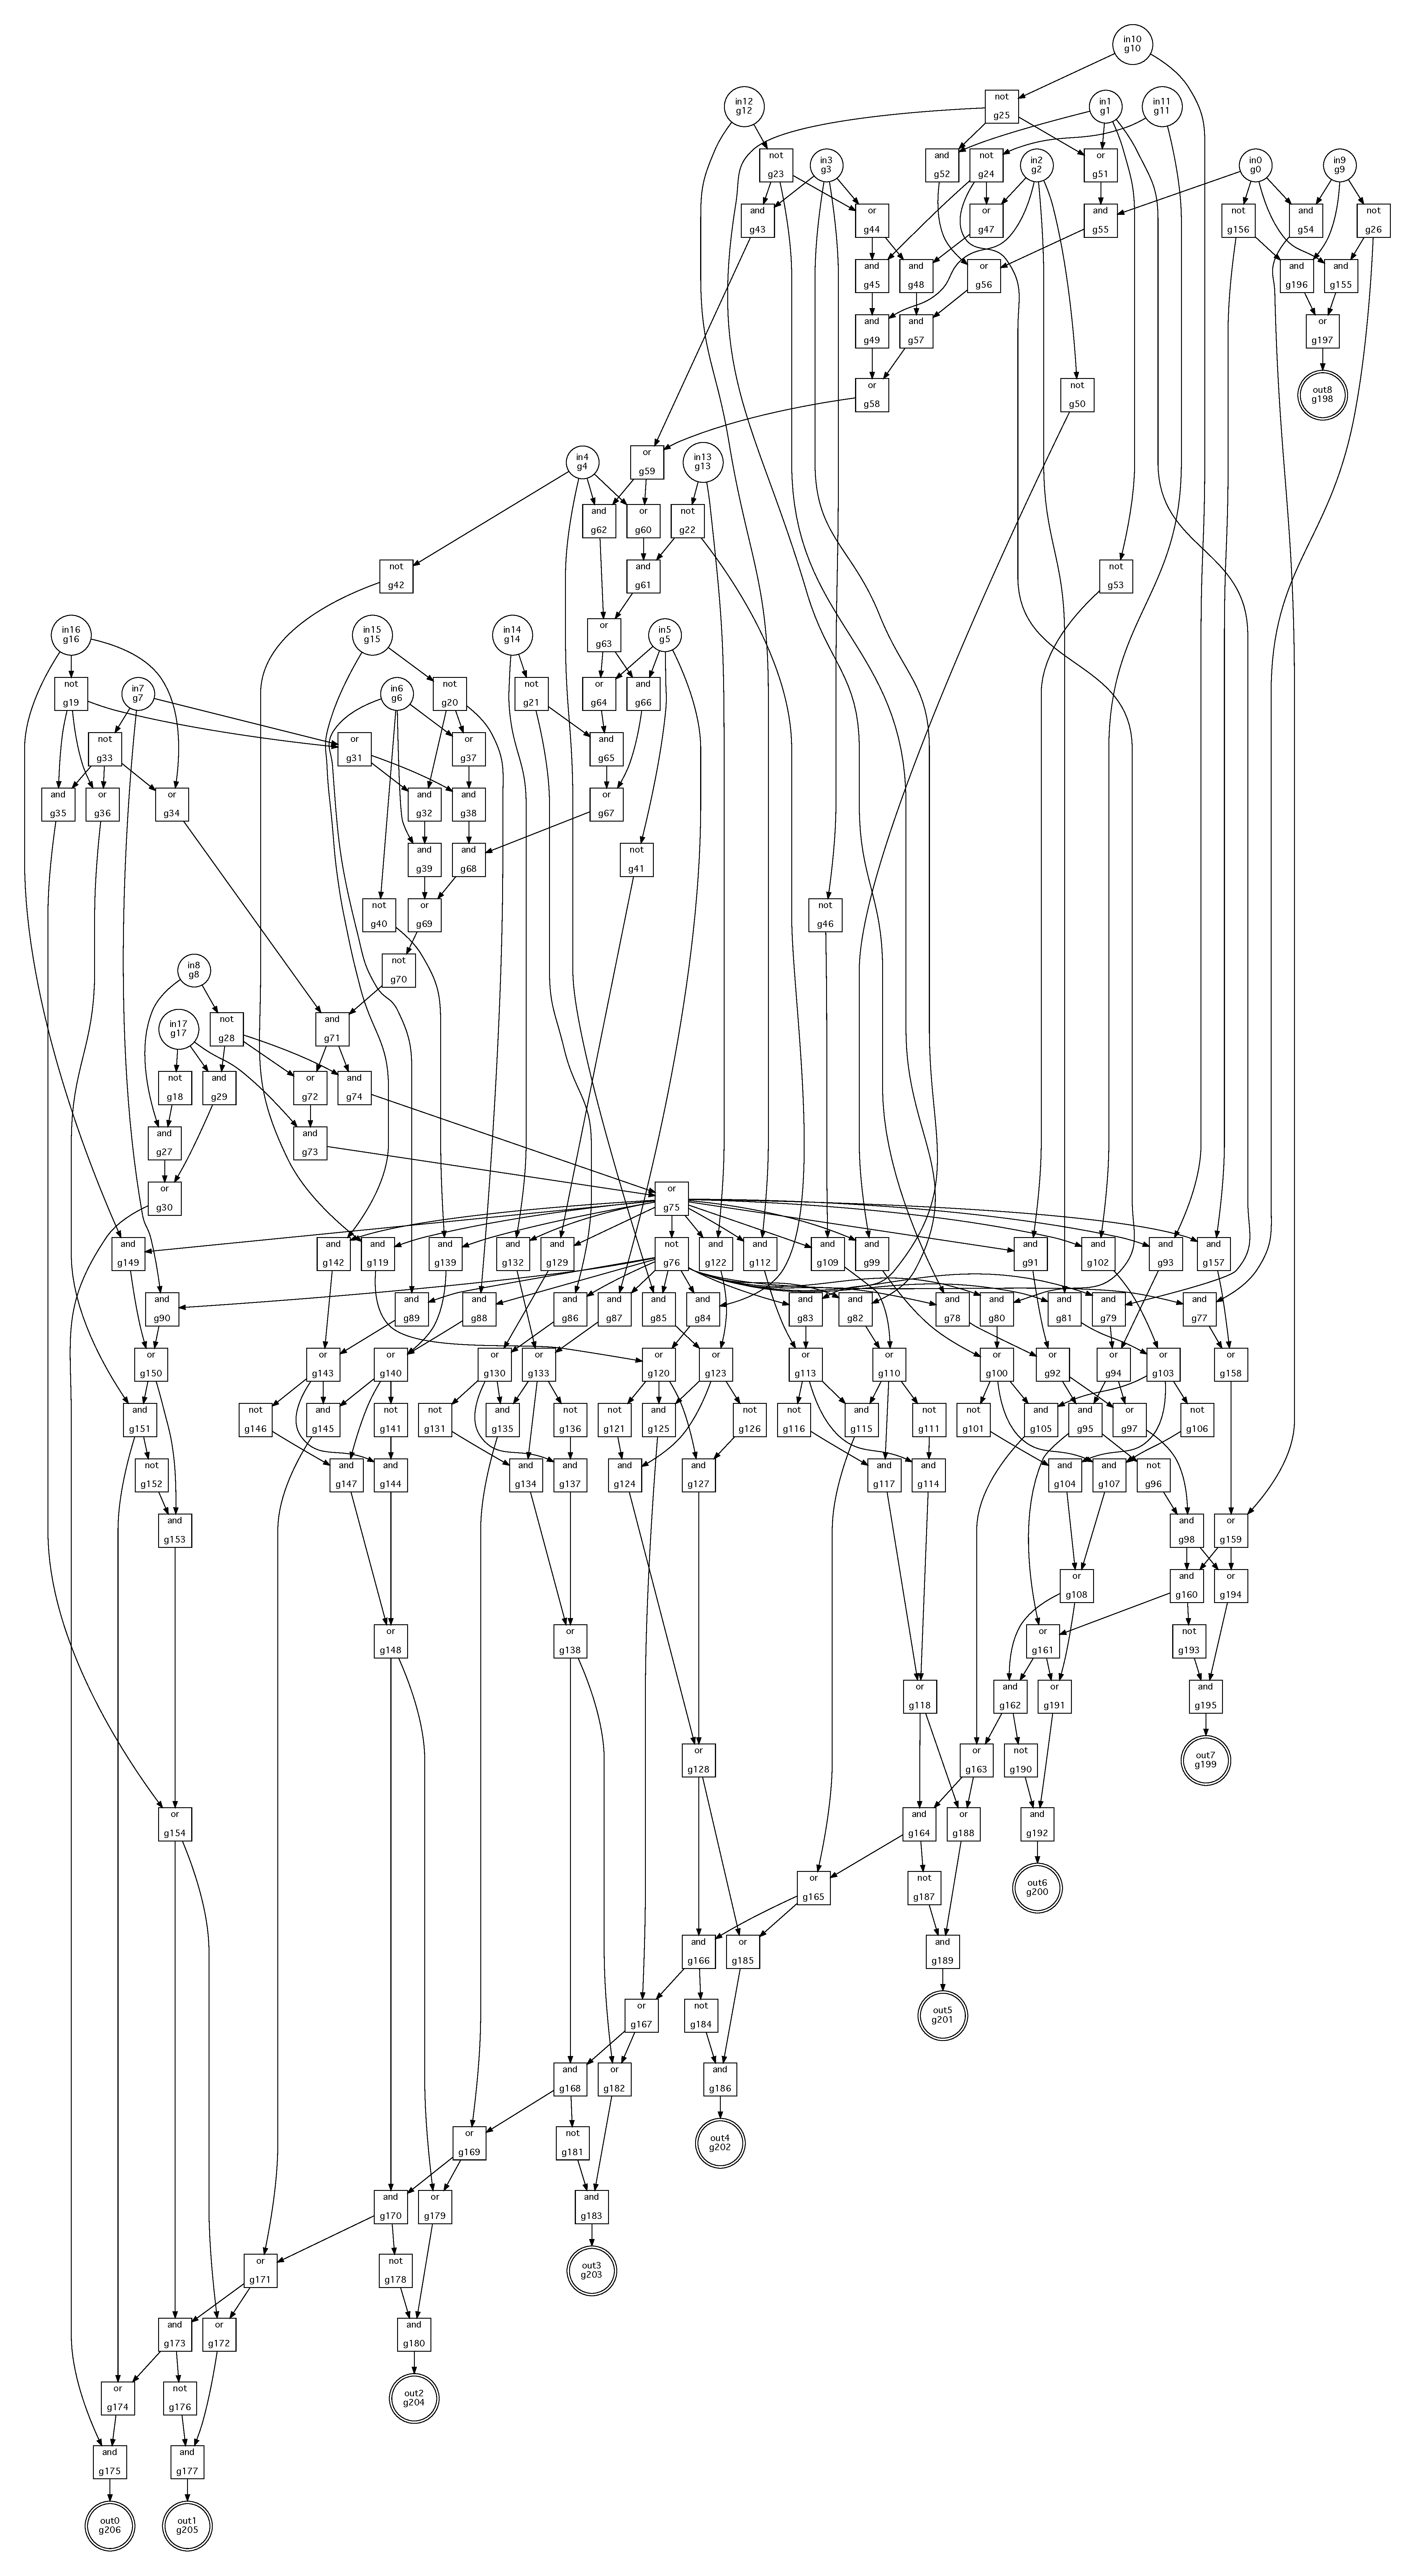
\includegraphics[width=10cm]{Results/abs_diff_9.pdf}
            \caption{\texttt{abs\_diff\_9} MUSes areas}
            \label{fig:r2}
        \end{figure}
    \item \texttt{\textbf{adder\_4bit}}\\
        The benchmark \texttt{adder\_4bit} has an exact area of $54.44$, a number of constraints of $46$, and the maximum value for error is $31$. \textbf{Table ~\ref{tab:r3}} and \textbf{Figure ~\ref{fig:r3}} display the obtained results for \texttt{adder\_4bit}.
        \begin{table}[H]
            \centering
            \begin{tabular}{c|c|c}
                \textbf{Error Threshold} & \textbf{\# MUSes} & \textbf{Minimal Area} \\ \hline
                3 & 2 & 38 \\
                \hline
                7 & 4 & 23 \\
                \hline
                11 & 11 & 19.24 \\
                \hline
                15 & 6 & 7.51 \\
                \hline
                19 & 22 & 7.51 \\
                \hline
                23 & 15 & 2.82    
            \end{tabular}
            \caption{\texttt{adder\_4} smallest MUSes areas}
            \label{tab:r3}
        \end{table}
        \begin{figure}[H]
            \centering
            \includegraphics[width=10cm]{Results/adder_4.pdf}
            \caption{\texttt{adder\_4} MUSes areas}
            \label{fig:r3}
        \end{figure}
    \item \texttt{\textbf{adder\_5bit}}\\
        The benchmark \texttt{adder\_5bit} has an exact area of $74.62$, a number of constraints of $57$, and the maximum value for error is $63$. \textbf{Table ~\ref{tab:r4}} and \textbf{Figure ~\ref{fig:r4}} display the obtained results for \texttt{adder\_5bit}.
        \begin{table}[H]
            \centering
            \begin{tabular}{c|c|c}
                \textbf{Error Threshold} & \textbf{\# MUSes} & \textbf{Minimal Area} \\ \hline
                7 & 14 & 34.73 \\
                \hline
                15 & 52 & 19.24 \\
                \hline
                23 & 97 & 9.39 \\
                \hline
                31 & 124 & 5.63 \\
                \hline
                39 & 231 & 5.63 \\
                \hline
                47 & 221 & 2.82    
            \end{tabular}
            \caption{\texttt{adder\_5\_0.3} smallest MUSes areas}
            \label{tab:r4}
        \end{table}
        \begin{figure}[H]
            \centering
            \includegraphics[width=10cm]{Results/adder_5_0.3.pdf}
            \caption{\texttt{adder\_5\_0.3} MUSes areas}
            \label{fig:r4}
        \end{figure}
    \item \texttt{\textbf{adder\_6bit}}\\
        The benchmark \texttt{adder\_6bit} has an exact area of $84.47$, a number of constraints of $79$, and the maximum value for error is $127$. \textbf{Table ~\ref{tab:r5}} and \textbf{Figure ~\ref{fig:r5}} display the obtained results for \texttt{adder\_6bit}.
        \begin{table}[H]
            \centering
            \begin{tabular}{c|c|c}
                \textbf{Error Threshold} & \textbf{\# MUSes} & \textbf{Minimal Area} \\ \hline
                15 & 75 & 31.91 \\
                \hline
                31 & 138 & 22.06 \\
                \hline
                47 & 138 & 14.08 \\
                \hline
                63 & 223 & 2.82 \\
                \hline
                79 & 376 & 2.82 \\
                \hline
                95 & 136 & 2.82    
            \end{tabular}
            \caption{\texttt{adder\_6\_0.3} smallest MUSes areas}
            \label{tab:r5}
        \end{table}
        \begin{figure}[H]
            \centering
            \includegraphics[width=10cm]{Results/adder_6_0.3.pdf}
            \caption{\texttt{adder\_6\_0.3}  MUSes areas}
            \label{fig:r5}
        \end{figure}
    \item \texttt{\textbf{adder\_8bit}}\\
        The benchmark \texttt{adder\_8bit} has an exact area of $115.92$, a number of constraints of $99$, and the maximum value for error is $511$. \textbf{Table ~\ref{tab:r6}} and \textbf{Figure ~\ref{fig:r6}} display the obtained results for \texttt{adder\_8bit}.
        \begin{table}[H]
            \centering
            \begin{tabular}{c|c|c}
                \textbf{Error Threshold} & \textbf{\# MUSes} & \textbf{Minimal Area} \\ \hline
                63 & 20 & 39.42 \\
                \hline
                127 & 24 & 22.53 \\
                \hline
                191 & 81 & 9.39 \\
                \hline
                255 & 28 & 7.51 \\
                \hline
                319 & 81 & 5.63 \\
                \hline
                383 & 63 & 2.82    
            \end{tabular}
            \caption{\texttt{adder\_8\_0.5} smallest MUSes areas}
            \label{tab:r6}
        \end{table}
        \begin{figure}[H]
            \centering
            \includegraphics[width=10cm]{Results/adder_8_0.5.pdf}
            \caption{\texttt{adder\_8\_0.5} MUSes areas}
            \label{fig:r6}
        \end{figure}
    \item \texttt{\textbf{multiply\_add\_3bit}}\\
        The benchmark \texttt{multiply\_add\_3bit} has an exact area of $127.65$, a number of constraints of $105$, and the maximum value for error is $63$. \textbf{Table ~\ref{tab:r7}} and \textbf{Figure ~\ref{fig:r7}} display the obtained results for \texttt{multiply\_add\_3bit}.
        \begin{table}[H]
            \centering
            \begin{tabular}{c|c|c}
                \textbf{Error Threshold} & \textbf{\# MUSes} & \textbf{Minimal Area} \\ \hline
                7 & 165 & 56.79 \\
                \hline
                15 & 200 & 28.63 \\
                \hline
                23 & 220 & 8.45 \\
                \hline
                31 & 306 & 8.45 \\
                \hline
                39 & 314 & 8.45 \\
                \hline
                47 & 215 & 2.82    
            \end{tabular}
            \caption{\texttt{madd\_3} smallest MUSes areas}
            \label{tab:r7}
        \end{table}
        \begin{figure}[H]
            \centering
            \includegraphics[width=10cm]{Results/madd_3.pdf}
            \caption{\texttt{madd\_3} MUSes areas}
            \label{fig:r7}
        \end{figure}
    \item \texttt{\textbf{multiplier\_6bit}}\\
        The benchmark \texttt{multiplier\_6bit} has an exact area of $481.5$, a number of constraints of $355$, and the maximum value for error is $4095$. \textbf{Table ~\ref{tab:r8}} and \textbf{Figure ~\ref{fig:r8}} display the obtained results for \texttt{multiplier\_6bit}.
        \begin{table}[H]
            \centering
            \begin{tabular}{c|c|c}
                \textbf{Error Threshold} & \textbf{\# MUSes} & \textbf{Minimal Area} \\ \hline
                511 & 15 & 152.52 \\
                \hline
                1023 & 62 & 63.36 \\
                \hline
                1535 & 63 & 22.53 \\
                \hline
                2047 & 143 & 8.45 \\
                \hline
                2559 & 78 & 8.45 \\
                \hline
                3071 & 221 & 2.82    
            \end{tabular}
            \caption{\texttt{mul\_6} smallest MUSes areas}
            \label{tab:r8}
        \end{table}
        \begin{figure}[H]
            \centering
            \includegraphics[width=10cm]{Results/mul_6.pdf}
            \caption{\texttt{mul\_6} MUSes areas}
            \label{fig:r8}
        \end{figure}
    \item \texttt{\textbf{online\_adder\_4bit}}\\
        The benchmark \texttt{online\_adder\_4bit} has an exact area of $127.65$, a number of constraints of $119$, and the maximum value for error is $1023$. \textbf{Table ~\ref{tab:r9}} and \textbf{Figure ~\ref{fig:r9}} display the obtained results for \texttt{online\_adder\_4bit}.
        \begin{table}[H]
            \centering
            \begin{tabular}{c|c|c}
                \textbf{Error Threshold} & \textbf{\# MUSes} & \textbf{Minimal Area} \\ \hline
                127 & 1 & 54.91 \\
                \hline
                255 & 1 & 30.5 \\
                \hline
                383 & 17 & 28.63 \\
                \hline
                511 & 1 & 7.04 \\
                \hline
                639 & 2 & 7.04 \\
                \hline
                767 & 2 & 7.04    
            \end{tabular}
            \caption{\texttt{online\_adder\_4} smallest MUSes areas}
            \label{tab:r9}
        \end{table}
        \begin{figure}[H]
            \centering
            \includegraphics[width=10cm]{Results/online_adder_4.pdf}
            \caption{\texttt{online\_adder\_4} MUSes areas}
            \label{fig:r9}
        \end{figure}
    \item \texttt{\textbf{online\_adder\_8bit}}\\
        The benchmark \texttt{online\_adder\_8bit} has an exact area of $254.83$, a number of constraints of $107$, and the maximum value for error is $262143$. \textbf{Table ~\ref{tab:r10}} and \textbf{Figure ~\ref{fig:r10}} display the obtained results for \texttt{online\_adder\_8bit}.
        \begin{table}[H]
            \centering
            \begin{tabular}{c|c|c}
                \textbf{Error Threshold} & \textbf{\# MUSes} & \textbf{Minimal Area} \\ \hline
                32767 & 1 & 55.85 \\
                \hline
                65535 & 1 & 30.5 \\
                \hline
                98303 & 11 & 28.63 \\
                \hline
                131071 & 1 & 7.04 \\
                \hline
                163839 & 2 & 7.04 \\
                \hline
                196607 & 2 & 7.04    
            \end{tabular}
            \caption{\texttt{online\_adder\_8} smallest MUSes areas}
            \label{tab:r10}
        \end{table}
        \begin{figure}[H]
            \centering
            \includegraphics[width=10cm]{Results/online_adder_8.pdf}
            \caption{\texttt{online\_adder\_8} MUSes areas}
            \label{fig:r10}
        \end{figure}
    \item \texttt{\textbf{sad\_4bit}}\\
        The benchmark \texttt{sad\_4bit} has an exact area of $438.8$, a number of constraints of $347$, and the maximum value for error is $31$. \textbf{Table ~\ref{tab:r11}} and \textbf{Figure ~\ref{fig:r11}} display the obtained results for \texttt{sad\_4bit}.
        \begin{table}[H]
            \centering
            \begin{tabular}{c|c|c}
                \textbf{Error Threshold} & \textbf{\# MUSes} & \textbf{Minimal Area} \\ \hline
                3 & 1 & 421.43 \\
                \hline
                7 & 1 & 409.7 \\
                \hline
                11 & 2 & 406.41 \\
                \hline
                15 & 1 & 402.66 \\
                \hline
                19 & 2 & 389.99 \\
                \hline
                23 & 2 & 380.13   
            \end{tabular}
            \caption{\texttt{sad\_4} smallest MUSes areas}
            \label{tab:r11}
        \end{table}
        \begin{figure}[H]
            \centering
            \includegraphics[width=10cm]{Results/sad_4.pdf}
            \caption{\texttt{sad\_4} MUSes areas}
            \label{fig:r11}
        \end{figure}
\end{itemize}
\newpage
\noindent
In order to better understand the differences between an exact circuit and one of its approximate versions, let us analyze a comparison between them, with an error threshold of $10$. \\
\textbf{Figure ~\ref{fig:exact}} and \textbf{Figure ~\ref{fig:approximate}} show the exact circuit and an approximate one of benchmark \texttt{adder\_4}, respectively. We can observe that many gates have been set to zero in the generated approximate circuit.
\begin{figure}[H]
    \centering
    \includegraphics[width=15cm]{assets/adder4.pdf}
    \caption{\texttt{adder\_4} exact circuit graphical representation}
    \label{fig:exact}
\end{figure}
\begin{figure}[H]
    \centering
    \includegraphics[width=17cm]{assets/adder_4.C10.pdf}
    \caption{\texttt{adder\_4} approximate circuit graphical representation (ET = 10)}
    \label{fig:approximate}
\end{figure}

\newpage

% -------------------------------------- %
% Chapter 5: Conclusions and Future Work
% -------------------------------------- %
\section{Conclusion and Future Work}\label{sec:conclusions}
% TODO: write some information about conclusions and future work concerning the Translator and the experiments
\subsection{Concluding Remarks}
In the first part of this project, we implemented a translator capable of converting \textit{blif} files into their corresponding version in the \textit{GV} format, while also simplifying them. Finally, the application generates a pdf file with dot, graphically rendering the circuit of the input file. The code and documentation of the \textit{Blif2GV Translator} can be found in its \textcolor{blue}{Github repository} \cite{gh}. \\
In the second part of this project, we performed various experiment on a set of different benchmarks by using \textit{MUST}, along with some constraints. We observed that \textit{MUST} is capable of rapidly synthesizing small approximate circuits. This proves the efficiency of SAT-based approximate synthesis, and leaves room for further exploration of the topic. \\
The \textit{Blif2GV Translator} was also helpful in this second part since, after generating a series of \textit{blif} files representing the approximate circuits of the input file, we could use it in order to display the exact circuit and all the approximate ones, getting a clear graphical view of the differences between them as shown in \textbf{Figure ~\ref{fig:exact}} and \textbf{Figure ~\ref{fig:approximate}}.
\subsection{Future Work}
One possible future enhancement of the \textit{Blif2GV Translator} could be integrating it into other tools for approximate logic synthesis. For example, we could develop an "\textit{approximate circuit visualization}" tool that takes approximate circuits written in the \textit{verilog} format, transforms them into their \textit{blif} counterparts with the \textit{abc} tool, and finally converts the newly-obtained files into \textit{GV} through the \textit{Blif2GV Translator}. \\
For what concerns the second part of this project (i.e., analysis on MUSes), after having quantified the approximate circuits' areas, we could compare the obtained results with those returned by other methods of the state of the art in order to assert on MUST effectiveness. Moreover, we could think of possible heuristics to improve MUST scalability for large circuits (e.g., 64-bit adders). Indeed, MUST is currently incapable to deal with such circuits and, hence, the relaxation of optimality requirements could represent a valid strategy.

\newpage

% ----------------------------- %
% Appendix A: Boolean Operators
% ----------------------------- %
\section{Appendix A - Boolean Operators}\label{sec:operators}
\subsection{Definition of Boolean Unary Operators}\label{subsubsec:definition-of-boolean-unary-operators}
A \textit{Boolean unary operation} consists of a single input, a \textit{unary operator}, and a single output. In order to better understand what a Boolean unary operator looks like, let us examine the following example:
\begin{center}
    $\Phi \ = \ (\neg x_1)$
\end{center}
The Boolean operator $\neg$ is known as "NOT" and, in this case, takes in input variable $x_1$, processes it, and returns a single output. \\
The following list explains the working of all the logical unary operators:
\begin{itemize}
    \item \textbf{ZERO} (unary)
        \vspace{0.2cm} \\
        The unary ZERO operator takes an input $x$ and returns \textcolor{red}{false}, regardless of the value of $x$:
        \begin{center}
            ZERO$_1(x) \ = \ \textcolor{red}{0}$
        \end{center}
        The subscript "$_1$" is needed to distinguish between the unary ZERO operator and the binary one. \\
        \textbf{Table ~\ref{tab:zero-unary-table}} shows the truth table of the unary ZERO operator.
        \begin{table}[H]
            \centering
            \begin{tabular}{|c|c|}
                \hline
                \textbf{Input} & \textbf{Output} \\
                \hline
                0 & \textcolor{red}{0} \\
                \hline
                1 & \textcolor{red}{0} \\
                \hline
            \end{tabular}
            \caption{Unary ZERO operator truth table}
            \label{tab:zero-unary-table}
        \end{table}
    \item \textbf{ASSIGN}
        \vspace{0.2cm} \\
        The ASSIGN operator takes an input $x$ and returns \textcolor{ForestGreen}{true} if the value of $x$ is \textcolor{ForestGreen}{true} or \textcolor{red}{false} if the value of $x$ is \textcolor{red}{false}:
        \begin{center}
            ASSIGN$(x) \ = \ x$
        \end{center}
        It is typically used to rename the input without changing its value. \\
        \textbf{Table ~\ref{tab:assign-table}} shows the truth table of the ASSIGN operator.
        \begin{table}[H]
            \centering
            \begin{tabular}{|c|c|}
                \hline
                \textbf{Input} & \textbf{Output} \\
                \hline
                0 & \textcolor{red}{0} \\
                \hline
                1 & \textcolor{ForestGreen}{1} \\
                \hline
            \end{tabular}
            \caption{ASSIGN operator truth table}
            \label{tab:assign-table}
        \end{table}
    \item \textbf{NOT}
        \vspace{0.2cm} \\
        The NOT operator takes an input $x$ and returns the complement of $x$; thus, it returns \textcolor{ForestGreen}{true} if the value of $x$ is \textcolor{red}{false} or \textcolor{red}{false} if the value of $x$ is \textcolor{ForestGreen}{true}:
        \begin{center}
            $\neg x \ = \ \overline{x}$
        \end{center}
        It is equivalent to the negated form of the ASSIGN operator:
        \begin{center}
            $\neg x \ \ \Longleftrightarrow \ \ \neg($ASSIGN$(x))$
        \end{center}
        \textbf{Table ~\ref{tab:not-table}} shows the truth table of the NOT operator.
        \begin{table}[H]
            \centering
            \begin{tabular}{|c|c|}
                \hline
                \textbf{Input} & \textbf{Output} \\
                \hline
                0 & \textcolor{ForestGreen}{1} \\
                \hline
                1 & \textcolor{red}{0} \\
                \hline
            \end{tabular}
            \caption{NOT operator truth table}
            \label{tab:not-table}
        \end{table}
    \item \textbf{ONE}
        \vspace{0.2cm} \\
        The unary ONE operator takes an input $x$ and returns \textcolor{ForestGreen}{true}, regardless of the value of $x$:
        \begin{center}
            ONE$_1(x) \ = \ \textcolor{ForestGreen}{1}$
        \end{center}
        The subscript "$_1$" is needed to distinguish between the unary ONE operator and the binary one. \\
        It is equivalent to the negated form of the unary ZERO operator:
        \begin{center}
            ONE$_1(x) \ \ \Longleftrightarrow \ \ \neg($ZERO$_1(x))$
        \end{center}
        \textbf{Table ~\ref{tab:one-unary-table}} shows the truth table of the unary ONE operator.
        \begin{table}[H]
            \centering
            \begin{tabular}{|c|c|}
                \hline
                \textbf{Input} & \textbf{Output} \\
                \hline
                0 & \textcolor{ForestGreen}{1} \\
                \hline
                1 & \textcolor{ForestGreen}{1} \\
                \hline
            \end{tabular}
            \caption{Unary ONE operator truth table}
            \label{tab:one-unary-table}
        \end{table}
\end{itemize}

\subsection{Definition of Boolean Binary Operators}\label{subsubsec:definition-of-boolean-binary-operators}
A \textit{Boolean binary operation} consists of two inputs, a \textit{binary operator}, and a single output. In order to better understand what a Boolean binary operator looks like, let us examine the following example:
\begin{center}
    $\Phi \ = \ (x_1 \ \land \ x_2)$
\end{center}
The Boolean operator $\land$ is known as "AND" and, in this case, takes in input variables $x_1$ and $x_2$, processes them, and returns a single output. \\
The following list explains the working of all the logical binary operators:
\begin{itemize}
    \item \textbf{ZERO} (binary)
        \vspace{0.2cm} \\
        The binary ZERO operator takes two inputs, $x$ and $y$, and returns \textcolor{red}{false}, regardless of the values of both $x$ and $y$:
        \begin{center}
            ZERO$_2(x, y) \ =\ \textcolor{red}{0}$
        \end{center}
        The subscript "$_2$" is needed to distinguish between the binary ZERO operator and the unary one. \\
        \textbf{Table ~\ref{tab:zero-table}} shows the truth table of the binary ZERO operator.
        \begin{table}[H]
            \centering
            \begin{tabular}{|c|c|c|}
                \hline
                \textbf{Input 1} & \textbf{Input 2} & \textbf{Output} \\
                \hline
                0 & 0 & \textcolor{red}{0} \\
                \hline
                0 & 1 & \textcolor{red}{0} \\
                \hline
                1 & 0 & \textcolor{red}{0} \\
                \hline
                1 & 1 & \textcolor{red}{0} \\
                \hline
            \end{tabular}
            \caption{Binary ZERO operator truth table}
            \label{tab:zero-table}
        \end{table}
    \item \textbf{AND}
        \vspace{0.2cm} \\
        The AND operator takes two inputs, $x$ and $y$, and returns \textcolor{ForestGreen}{true} only if the values of $x$ and $y$ are both \textcolor{ForestGreen}{true}; otherwise, it returns \textcolor{red}{false}:
        \begin{center}
            $x \ \land \ y$
        \end{center}
        \textbf{Table ~\ref{tab:and-table}} shows the truth table of the AND operator.
        \begin{table}[H]
            \centering
            \begin{tabular}{|c|c|c|}
                \hline
                \textbf{Input 1} & \textbf{Input 2} & \textbf{Output} \\ \hline
                0 & 0 & \textcolor{red}{0} \\
                \hline
                0 & 1 & \textcolor{red}{0} \\
                \hline
                1 & 0 & \textcolor{red}{0} \\
                \hline
                1 & 1 & \textcolor{ForestGreen}{1} \\
                \hline
            \end{tabular}
            \caption{AND operator truth table}
            \label{tab:and-table}
        \end{table}
    \item \textbf{NOT\_IMPLY}
        \vspace{0.2cm} \\
        The NOT\_IMPLY operator takes two inputs, $x$ and $y$, and returns \textcolor{ForestGreen}{true} only if the values of $x$ and $y$ are \textcolor{ForestGreen}{true} and \textcolor{red}{false}, respectively; otherwise, it returns \textcolor{red}{false}:
        \begin{center}
            $x \ \ \overline{\Longrightarrow} \ \ y$
        \end{center}
        It is equivalent to the negated form of the IMPLY operator:
        \begin{center}
            $x \ \ \overline{\Longrightarrow} \ \ y \ \ \Longleftrightarrow \ \ \neg(x \ \Longrightarrow \ y)$
        \end{center}
        \textbf{Table ~\ref{tab:not-imply-table}} shows the truth table of the NOT\_IMPLY operator.
        \begin{table}[H]
            \centering
            \begin{tabular}{|c|c|c|}
                \hline
                \textbf{Input 1} & \textbf{Input 2} & \textbf{Output} \\ \hline
                0 & 0 & \textcolor{red}{0} \\
                \hline
                0 & 1 & \textcolor{red}{0} \\
                \hline
                1 & 0 & \textcolor{ForestGreen}{1} \\
                \hline
                1 & 1 & \textcolor{red}{0} \\
                \hline
            \end{tabular}
            \caption{NOT\_IMPLY operator truth table}
            \label{tab:not-imply-table}
        \end{table}
    \item \textbf{ONE\_DC}
        \vspace{0.2cm} \\
        The ONE\_DC operator takes two inputs, $x$ and $y$, and returns \textcolor{ForestGreen}{true} only if the value of the first input (i.e., $x$) is \textcolor{ForestGreen}{true}, regardless of the value of the second input (i.e., $y$); otherwise, it returns \textcolor{red}{false}:
        \begin{center}
            ONE\_DC$(\textcolor{ForestGreen}{x}, y) \ = \ \textcolor{ForestGreen}{x}$
        \end{center}
        \textbf{Table ~\ref{tab:one-dc-table}} shows the truth table of the ONE\_DC operator.
        \begin{table}[H]
            \centering
            \begin{tabular}{|c|c|c|}
                \hline
                \textbf{Input 1} & \textbf{Input 2} & \textbf{Output} \\ \hline
                0 & 0 & \textcolor{red}{0} \\
                \hline
                0 & 1 & \textcolor{red}{0} \\
                \hline
                1 & 0 & \textcolor{ForestGreen}{1} \\
                \hline
                1 & 1 & \textcolor{ForestGreen}{1} \\
                \hline
            \end{tabular}
            \caption{ONE\_DC operator truth table}
            \label{tab:one-dc-table}
        \end{table}
    \item \textbf{ZERO\_ONE}
        \vspace{0.2cm} \\
        The ZERO\_ONE operator takes two inputs, $x$ and $y$, and returns \textcolor{ForestGreen}{true} only if the values of $x$ and $y$ are \textcolor{red}{false} and \textcolor{ForestGreen}{true}, respectively; otherwise, it returns \textcolor{red}{false}:
        \begin{center}
            ZERO\_ONE$(\textcolor{red}{x}, \textcolor{ForestGreen}{y})\ =\ \textcolor{ForestGreen}{1}$
        \end{center}
        \textbf{Table ~\ref{tab:zero-one-table}} shows the truth table of the ZERO\_ONE operator.
        \begin{table}[H]
            \centering
            \begin{tabular}{|c|c|c|}
                \hline
                \textbf{Input 1} & \textbf{Input 2} & \textbf{Output} \\ \hline
                0 & 0 & \textcolor{red}{0} \\
                \hline
                0 & 1 & \textcolor{ForestGreen}{1} \\
                \hline
                1 & 0 & \textcolor{red}{0} \\
                \hline
                1 & 1 & \textcolor{red}{0} \\
                \hline
            \end{tabular}
            \caption{ZERO\_ONE operator truth table}
            \label{tab:zero-one-table}
        \end{table}
    \item \textbf{DC\_ONE}
        \vspace{0.2cm} \\
        The DC\_ONE operator takes two inputs, $x$ and $y$, and returns \textcolor{ForestGreen}{true} only if the value of the second input (i.e., $y$) is \textcolor{ForestGreen}{true}, regardless of the value of the first input (i.e., $x$); otherwise, it returns \textcolor{red}{false}:
        \begin{center}
            DC\_ONE$(x,\textcolor{ForestGreen}{y})\ =\ \textcolor{ForestGreen}{1}$
        \end{center}
        \textbf{Table ~\ref{tab:dc-one-table}} shows the truth table of the DC\_ONE operator.
        \begin{table}[H]
            \centering
            \begin{tabular}{|c|c|c|}
                \hline
                \textbf{Input 1} & \textbf{Input 2} & \textbf{Output} \\
                \hline
                0 & 0 & \textcolor{red}{0} \\
                \hline
                0 & 1 & \textcolor{ForestGreen}{1} \\
                \hline
                1 & 0 & \textcolor{red}{0} \\
                \hline
                1 & 1 & \textcolor{ForestGreen}{1} \\
                \hline
            \end{tabular}
            \caption{DC\_ONE operator truth table}
            \label{tab:dc-one-table}
        \end{table}
    \item \textbf{XOR}
        \vspace{0.2cm} \\
        The XOR operator takes two inputs, $x$ and $y$, and returns \textcolor{ForestGreen}{true} only if exactly one of the values of $x$ and $y$ is \textcolor{ForestGreen}{true}; otherwise, it returns \textcolor{red}{false}:
        \begin{center}
            $x \ \oplus \ y$
        \end{center}
        \textbf{Table ~\ref{tab:xor-table}} shows the truth table of the XOR operator.
        \begin{table}[H]
            \centering
            \begin{tabular}{|c|c|c|}
                \hline
                \textbf{Input 1} & \textbf{Input 2} & \textbf{Output} \\
                \hline
                0 & 0 & \textcolor{red}{0} \\
                \hline
                0 & 1 & \textcolor{ForestGreen}{1} \\
                \hline
                1 & 0 & \textcolor{ForestGreen}{1} \\
                \hline
                1 & 1 & \textcolor{red}{0} \\
                \hline
            \end{tabular}
            \caption{XOR operator truth table}
            \label{tab:xor-table}
        \end{table}
    \item \textbf{OR}
        \vspace{0.2cm} \\
        The OR operator takes two inputs, $x$ and $y$, and returns \textcolor{ForestGreen}{true} only if at least one of the values of $x$ and $y$ is \textcolor{ForestGreen}{true}; otherwise, it returns \textcolor{red}{false}:
        \begin{center}
            $x \ \lor \ y$
        \end{center}
        \textbf{Table ~\ref{tab:or-table}} shows the truth table of the OR operator.
        \begin{table}[H]
            \centering
            \begin{tabular}{|c|c|c|}
                \hline
                \textbf{Input 1} & \textbf{Input 2} & \textbf{Output} \\
                \hline
                0 & 0 & \textcolor{red}{0} \\
                \hline
                0 & 1 & \textcolor{ForestGreen}{1} \\
                \hline
                1 & 0 & \textcolor{ForestGreen}{1} \\
                \hline
                1 & 1 & \textcolor{ForestGreen}{1} \\
                \hline
            \end{tabular}
            \caption{OR operator truth table}
            \label{tab:or-table}
        \end{table}
    \item \textbf{NOR}
        \vspace{0.2cm} \\
        The NOR operator takes two inputs, $x$ and $y$, and returns \textcolor{ForestGreen}{true} only if both the values of $x$ and $y$ are \textcolor{red}{false}; otherwise, it returns \textcolor{red}{false}:
        \begin{center}
            $x \ \overline{\lor} \ y$
        \end{center}
        It is equivalent to the negated form of the OR operator:
        \begin{center}
            $x \ \overline{\lor} \ y \ \ \Longleftrightarrow \ \ \neg(x \ \lor \ y)$
        \end{center}
        \textbf{Table ~\ref{tab:nor-table}} shows the truth table of the NOR operator.
        \begin{table}[H]
            \centering
            \begin{tabular}{|c|c|c|}
                \hline
                \textbf{Input 1} & \textbf{Input 2} & \textbf{Output} \\
                \hline
                0 & 0 & \textcolor{ForestGreen}{1} \\
                \hline
                0 & 1 & \textcolor{red}{0} \\
                \hline
                1 & 0 & \textcolor{red}{0} \\
                \hline
                1 & 1 & \textcolor{red}{0} \\
                \hline
            \end{tabular}
            \caption{NOR operator truth table}
            \label{tab:nor-table}
        \end{table}
    \item \textbf{EQUALITY}
        \vspace{0.2cm} \\
        The EQUALITY operator takes two inputs, $x$ and $y$, and returns \textcolor{ForestGreen}{true} only if the values of $x$ and $y$ are equal (i.e., they are both \textcolor{ForestGreen}{true} or \textcolor{red}{false}); otherwise, it returns \textcolor{red}{false}:
        \begin{center}
            $x \ \Longleftrightarrow \ y$
        \end{center}
        It is equivalent to the negated form of the XOR operator:
        \begin{center}
            $(x \ \Longleftrightarrow \ y) \ \ \Longleftrightarrow \ \ \neg(x \ \oplus \ y)$
        \end{center}
        \textbf{Table ~\ref{tab:equality-table}} shows the truth table of the EQUALITY operator.
        \begin{table}[H]
            \centering
            \begin{tabular}{|c|c|c|}
                \hline
                \textbf{Input 1} & \textbf{Input 2} & \textbf{Output} \\
                \hline
                0 & 0 & \textcolor{ForestGreen}{1} \\ 
                \hline
                0 & 1 & \textcolor{red}{0} \\ 
                \hline
                1 & 0 & \textcolor{red}{0} \\ 
                \hline
                1 & 1 & \textcolor{ForestGreen}{1} \\ 
                \hline
            \end{tabular}
            \caption{EQUALITY operator truth table}
            \label{tab:equality-table}
        \end{table}
    \item \textbf{DC\_ZERO}
        \vspace{0.2cm} \\
        The DC\_ZERO operator takes two inputs, $x$ and $y$, and returns \textcolor{ForestGreen}{true} only if the value of the second input (i.e., $y$) is \textcolor{red}{false}, regardless of the value of the first input (i.e., $x$); otherwise, it returns \textcolor{red}{false}:
        \begin{center}
            DC\_ZERO$(x,\textcolor{red}{y}) \ = \ \textcolor{ForestGreen}{1}$
        \end{center}
        It is equivalent to the negated form of the DC\_ONE operator:
        \begin{center}
            DC\_ZERO$(x,y) \ \ \Longleftrightarrow \ \ \neg($DC\_ONE$(x,y))$
        \end{center}
        \textbf{Table ~\ref{tab:dc-zero-table}} shows the truth table of the DC\_ZERO operator.
        \begin{table}[H]
            \centering
            \begin{tabular}{|c|c|c|}
                \hline
                \textbf{Input 1} & \textbf{Input 2} & \textbf{Output} \\
                \hline
                0 & 0 & \textcolor{ForestGreen}{1} \\
                \hline
                0 & 1 & \textcolor{red}{0} \\
                \hline
                1 & 0 & \textcolor{ForestGreen}{1} \\
                \hline
                1 & 1 & \textcolor{red}{0} \\
                \hline
            \end{tabular}
            \caption{DC\_ZERO operator truth table}
            \label{tab:dc-zero-table}
        \end{table}
    \item \textbf{NOT\_ZERO\_ONE}
        \vspace{0.2cm} \\
        The NOT\_ZERO\_ONE operator takes two inputs, $x$ and $y$, and returns \textcolor{red}{false} only if the values of $x$ and $y$ are \textcolor{red}{false} and \textcolor{ForestGreen}{true}, respectively; otherwise, it returns \textcolor{ForestGreen}{true}:
        \begin{center}
            NOT\_ZERO\_ONE$(\textcolor{red}{x},\textcolor{ForestGreen}{y})\ =\ \textcolor{red}{0}$
        \end{center}
        It is equivalent to the negated form of the ZERO\_ONE operator:
        \begin{center}
            NOT\_ZERO\_ONE$(x,y) \ \ \Longleftrightarrow \ \ \neg($ZERO\_ONE$(x,y))$
        \end{center}
        \textbf{Table ~\ref{tab:dc-zero-table}} shows the truth table of the NOT\_ZERO\_ONE operator.
        \begin{table}[H]
            \centering
            \begin{tabular}{|c|c|c|}
                \hline
                \textbf{Input 1} & \textbf{Input 2} & \textbf{Output} \\
                \hline
                0 & 0 & \textcolor{ForestGreen}{1} \\ 
                \hline
                0 & 1 & \textcolor{red}{0} \\
                \hline
                1 & 0 & \textcolor{ForestGreen}{1} \\
                \hline
                1 & 1 & \textcolor{ForestGreen}{1} \\ 
                \hline
            \end{tabular}
            \caption{NOT\_ZERO\_ONE operator truth table}
            \label{tab:not-zero-one-table}
        \end{table}
    \item \textbf{ZERO\_DC}
        \vspace{0.2cm} \\
        The ZERO\_DC operator takes two inputs, $x$ and $y$, and returns \textcolor{ForestGreen}{true} only if the value of the first input (i.e., $x$) is \textcolor{red}{false}, regardless of the value of the second input (i.e., $y$); otherwise, it returns \textcolor{red}{false}:
        \begin{center}
            ZERO\_DC$(\textcolor{red}{x}, y) \ =\ \textcolor{ForestGreen}{1}$
        \end{center}
        It is equivalent to the negated form of the ONE\_DC operator:
        \begin{center}
            ZERO\_DC$(x,y) \ \ \Longleftrightarrow \ \ \neg($ONE\_DC$(x,y))$
        \end{center}
        \textbf{Table ~\ref{tab:zero-dc-table}} shows the truth table of the ZERO\_DC operator.
        \begin{table}[H]
            \centering
            \begin{tabular}{|c|c|c|}
                \hline
                \textbf{Input 1} & \textbf{Input 2} & \textbf{Output} \\
                \hline
                0 & 0 & \textcolor{ForestGreen}{1} \\
                \hline
                0 & 1 & \textcolor{ForestGreen}{1} \\
                \hline
                1 & 0 & \textcolor{red}{0} \\
                \hline
                1 & 1 & \textcolor{red}{0} \\
                \hline
            \end{tabular}
            \caption{ZERO\_DC operator truth table}
            \label{tab:zero-dc-table}
        \end{table}
    \item \textbf{IMPLY}
        \vspace{0.2cm} \\
        The IMPLY operator takes two inputs, $x$ and $y$, and returns \textcolor{red}{false} only if the values of $x$ and $y$ are \textcolor{ForestGreen}{true} and \textcolor{red}{false}, respectively; otherwise, it returns \textcolor{ForestGreen}{true}:
        \begin{center}
            $x \ \Longrightarrow \ y$
        \end{center}
        \textbf{Table ~\ref{tab:imply-table}} shows the truth table of the IMPLY operator.
        \begin{table}[H]
            \centering
            \begin{tabular}{|c|c|c|}
                \hline
                \textbf{Input 1} & \textbf{Input 2} & \textbf{Output} \\
                \hline
                0 & 0 & \textcolor{ForestGreen}{1} \\
                \hline
                0 & 1 & \textcolor{ForestGreen}{1} \\
                \hline
                1 & 0 & \textcolor{red}{0} \\
                \hline
                1 & 1 & \textcolor{ForestGreen}{1} \\
                \hline
            \end{tabular}
            \caption{IMPLY operator truth table}
            \label{tab:imply-table}
        \end{table}
    \item \textbf{NAND}
        \vspace{0.2cm} \\
        The NAND operator takes two inputs, $x$ and $y$, and returns \textcolor{red}{false} if the values of $x$ and $y$ are both \textcolor{ForestGreen}{true}; otherwise, it returns \textcolor{ForestGreen}{true}:
        \begin{center}
            $x \ \overline{\land} \ y$
        \end{center}
        It is equivalent to the negated form of the AND operator:
        \begin{center}
            $x \ \overline{\land} \ y \ \ \Longleftrightarrow \ \ \neg(x \ \land \ y)$
        \end{center}
        \textbf{Table ~\ref{tab:nand-table}} shows the truth table of the NAND operator.
        \begin{table}[H]
            \centering
            \begin{tabular}{|c|c|c|}
                \hline
                \textbf{Input 1} & \textbf{Input 2} & \textbf{Output} \\
                \hline
                0 & 0 & \textcolor{ForestGreen}{1} \\
                \hline
                0 & 1 & \textcolor{ForestGreen}{1} \\
                \hline
                1 & 0 & \textcolor{ForestGreen}{1} \\
                \hline
                1 & 1 & \textcolor{red}{0} \\
                \hline
            \end{tabular}
            \caption{NAND operator truth table}
            \label{tab:nand-table}
        \end{table}
    \item \textbf{ONE} (binary)
        \vspace{0.2cm} \\
        The binary ONE operator takes two inputs, $x$ and $y$, and returns \textcolor{ForestGreen}{true}, regardless of the values of both $x$ and $y$:
        \begin{center}
            \begin{center}
                ONE$_2(x,y) \ =\ \textcolor{ForestGreen}{1}$
            \end{center}
        \end{center}
        The subscript "$_2$" is needed to distinguish between the binary ONE operator and the unary one. \\
        It is equivalent to the negated form of the binary ZERO operator:
        \begin{center}
            ONE$_2(x,y) \ \ \Longleftrightarrow \ \ \neg($ZERO$_2(x,y))$
        \end{center}
        \textbf{Table ~\ref{tab:one-table}} shows the truth table of the binary ONE operator.
        \begin{table}[H]
            \centering
            \begin{tabular}{|c|c|c|}
                \hline
                \textbf{Input 1} & \textbf{Input 2} & \textbf{Output} \\
                \hline
                0 & 0 & \textcolor{ForestGreen}{1} \\
                \hline
                0 & 1 & \textcolor{ForestGreen}{1} \\
                \hline
                1 & 0 & \textcolor{ForestGreen}{1} \\
                \hline
                1 & 1 & \textcolor{ForestGreen}{1} \\
                \hline
            \end{tabular}
            \caption{Binary ONE operator truth table}
            \label{tab:one-table}
        \end{table}
\end{itemize}

\newpage

% --------------------- %
% Extra 1: Bibliography
% --------------------- %
\bibliographystyle{unsrt}
\bibliography{references}

\end{document}